\documentclass{article}

% Use the Cactus ThornGuide style file
% (Automatically used from Cactus distribution, if you have a 
%  thorn without the Cactus Flesh download this from the Cactus
%  homepage at www.cactuscode.org)
\usepackage{../../../../doc/latex/cactus}

\begin{document}

\title{Using SpaceMask}
\author{Denis Pollney}
\date{$ $Date$ $}

\maketitle

% Do not delete next line
% START CACTUS THORNGUIDE

\begin{abstract}
The SpaceMask thorn provides a grid function which can be used to
store user-defined states at each grid point. Routines are provided
for quickly setting and checking the mask states.
\end{abstract}

\section{The mask bit-field}

The mask is a grid function which can be used to assign a state to
each point on the grid. It is used as a bit field, with different
bits, or combinations of bits, assigned to represent various states.
The mask is currently implemented as a CCTK\_INT grid function,
providing 32 bits per point.\footnote{The original implementation of
these functions used a CCTK\_INT8 for 64 bits, however this data type
is not supported by some Fortran compilers.} Appropriate numbers of
bits within the mask can be allocated to represent individual states
of a given type.

For instance, a programmer wants to record whether each point of the
grid has \emph{state} ``interior'', ``excised'' or ``boundary''. The
collection of these states is called a \emph{type}, and 2-bits of the
mask (enough to represent the three possible states of the type) are
allocated to hold this information. If an independent classification
of points (ie. a new type) is required, bits are allocated to it from
the remaining free bits in the mask. (See Figure \ref{fig:mask_bits}.)

The SpaceMask thorn provides a set of routines for allocating bits
within the mask, and for setting and checking the mask state at
individual points.

\begin{figure}
  \centering
  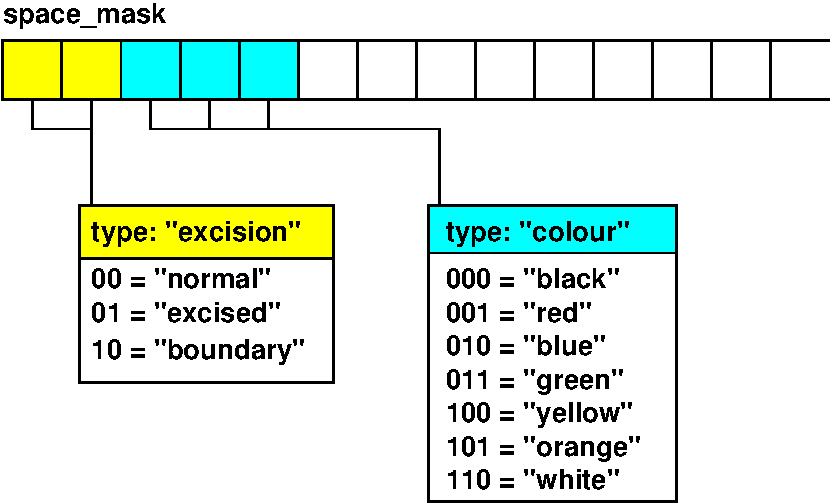
\includegraphics{space_mask}
  \caption{The \texttt{SpaceMask\_RegisterType()} function allocates
  bits of the mask to a new ``type'' (eg. ``excision'' and ``colour''
  in the figure). The number of bits that are allocated is determined
  by the number of possible states of the given type.}
  \label{fig:mask_bits}
\end{figure}

\section{Using the mask}

A number of functions are provided for registering new types, and
checking and setting mask values at a point. The interface to these
functions differs slightly for C and Fortran90 code.

\subsection{Accessing the mask from C Code}

The following description describes the C interface for manipulating
the mask. An example of code using these functions can be found in
Appendix \ref{app:eg_C}.

\subsubsection{Registering a new type}\label{sec:reg_C}

Bits of the mask are allocated to a new type using the function:

\indent\parbox{\linewidth}{
\vspace{\baselineskip}\noindent\texttt{
int SpaceMask\_RegisterType(const char* \emph{type\_name},
  \\\hspace*{10mm}
  int \emph{nstates}, const char* const \emph{state\_list}[])
}\\
\hspace*{10mm}\parbox{\linewidth}{
\begin{description}
  \item[\emph{type\_name}] The name of the new type to be registered;
  \item[\emph{nstates}] The number of states in the new type;
  \item[\emph{state\_list}] A list of names, one for each state, or NULL.
\end{description}
}
}

\noindent An appropriate number of bits of the mask are allocated to
hold a unique value for the $n$ states specified by the \emph{nstates}
argument. The registration must take place before the type can be
used, so for instance, this could be scheduled at CCTK\_STARTUP. The
function returns a $-1$ if the required states cannot be allocated
(for example, if there are not enough free bits remaining in the
mask), otherwise it returns $0$.

It is possible to allocate a portion of the mask without assigning
names to any of the states by passing NULL as the \emph{state\_list}.
This is useful when some integer number of states is required for a
given type, but the number of states and appropriate names are not
known at compile time. States which are allocated in this way can be
accessed using the \texttt{SpaceMask\_GetStateBitsList()}.

New states can be added to an already allocated type using the
function:

\indent\parbox{\linewidth}{
\vspace{\baselineskip}\noindent\texttt{
int SpaceMask\_AppendStatesToType(const char* \emph{type\_name},
  \\\hspace*{10mm}
  int \emph{nstates}, const char* const \emph{state\_list}[])
}\\
\hspace*{10mm}\parbox{\linewidth}{
\begin{description}
  \item[\emph{type\_name}] The name of an already registered type;
  \item[\emph{nstates}] The number of states to be added;
  \item[\emph{state\_list}] A list of names, one for each of the new
    states.
\end{description}
}}

\noindent A number of new bits will be added to the specified type
appropriate to hold the number of existing states plus the extra
states. The allocated bits need not be contiguous within the mask.
The function returns $0$ if successful, otherwise a $-1$ if the new
states could not be allocated.


\subsubsection{Setting and checking mask states}

The state of the mask at a given point is set using the function:

\indent\parbox{\linewidth}{
\vspace{\baselineskip}\noindent\texttt{
void SpaceMask\_SetState(CCTK\_INT* \emph{mask}, int \emph{point},
  \\\hspace*{10mm}
  const char* \emph{type\_name}, const char* \emph{state})
}\\
\hspace*{10mm}\parbox{\linewidth}{
\begin{description}
  \item[\emph{mask}] A pointer to the mask grid function;
  \item[\emph{point}] The index of the point within the grid function
    array;
  \item[\emph{type\_name}] The name of the type containing the state;
  \item[\emph{state\_name}] The particular state to be set.
\end{description}
}}

The state of the mask at a given point can be checked using:

\indent\parbox{\linewidth}{
\vspace{\baselineskip}\noindent\texttt{
int SpaceMask\_CheckState(const CCTK\_INT* \emph{mask}, int \emph{point},
  \\\hspace*{10mm}
  const char* \emph{type\_name}, const char* \emph{state})
}\\
\hspace*{10mm}\parbox{\linewidth}{
\begin{description}
  \item[\emph{mask}] A pointer to the mask grid function;
  \item[\emph{point}] The index of the point within the grid function
    array;
  \item[\emph{type\_name}] The name of the type containing the state;
  \item[\emph{state\_name}] The particular state to be compared.
\end{description}
}}

The return value is 1 if the given \emph{state\_name} has been set at
the point, or 0 otherwise.

\subsubsection{Faster bitwise operators}

The above mentioned functions for checking and setting the mask are
rather inefficient, since they require strings to be compared at each
point. A set of faster macros are provided which operate on the mask
by performing bit operations directly. In order to use these
functions, the bitmasks corresponding to the desired type and it's
states need to be obtained using the following functions:

\indent\parbox{\linewidth}{
\vspace{\baselineskip}\noindent\texttt{
CCTK\_INT SpaceMask\_GetTypeBits(const char* \emph{type\_name})
}\\
\hspace*{10mm}\parbox{\linewidth}{
\begin{description}
  \item[\emph{type\_name}] The type for which the bitmask is to be
  determined.
\end{description}
}}

\indent\parbox{\linewidth}{
\vspace{\baselineskip}\noindent\texttt{
CCTK\_INT SpaceMask\_GetStateBits(const char* \emph{type\_name},
  const char* \emph{state\_name})
}
\hspace*{10mm}\parbox{\linewidth}{
\begin{description}
  \item[\emph{type\_name}] The type containing the state in question;
  \item[\emph{state\_name}] The state whose bitmask is to be determined.
\end{description}
}}

\noindent Each of these functions returns a CCTK\_INT8 which holds the
bitmask corresponding to the given type or state. For example, if a
given type uses three bits of the mask, the returned value could be
the integer corresponding to the bitfield $001110000$\ldots, where the
location of $1$s indicates the bits which have been allocated to the
given type. A return value of $0$ (GetTypeBits) or $-1$ (GetStateBits)
indicates that the bitmask could
not be determined for some reason (for example, the requested state
was not previously registered).

All of the state masks allocated for a given type can be retrieved
using the following function:

\indent\parbox{\linewidth}{
\vspace{\baselineskip}\noindent\texttt{
CCTK\_INT* SpaceMask\_GetStateBitsList(const char* \emph{type\_name})
}\\
\hspace*{10mm}\parbox{\linewidth}{
\begin{description}
  \item[\emph{type\_name}] The type for which the bitmask is to be
  determined.
\end{description}
}}

The return value is a list of integers, with a length corresponding to
the number of states of the given type. Each of the entries is a
bitmask which identifies the state. List entries are returned in the
order in which they were originally assigned. This allows for a simple
correspondence between states and integers (given by the index of the
list entry). \emph{A fortran wrapper does not currently exist for this
functionality.}

The following macros have been defined for fast setting and checking
of the mask by direct bitwise operations:

\indent\parbox{\linewidth}{
\vspace{\baselineskip}\noindent\texttt{
void SpaceMask\_SetStateBits(CCTK\_INT* \emph{mask}, int \emph{point},
  \\\hspace*{10mm}
  CCTK\_INT \emph{type\_bits}, CCTK\_INT \emph{state\_bits})
}\\
\hspace*{10mm}\parbox{\linewidth}{
\begin{description}
  \item[\emph{mask}] A pointer to the mask grid function;
  \item[\emph{point}] The index of the point within the grid function
    array;
  \item[\emph{type\_bits}] The bitmask corresponding to the required
    type;
  \item[\emph{state\_bits}] The bitmask corrsponding to the required
    state;
\end{description}
}}

\indent\parbox{\linewidth}{
\vspace{\baselineskip}\noindent\texttt{
int SpaceMask\_CheckStateBits(const CCTK\_INT* \emph{mask}, int \emph{point},
  \\\hspace*{10mm}
  CCTK\_INT \emph{type\_bits}, CCTK\_INT \emph{state\_bits})
}\\
\hspace*{10mm}\parbox{\linewidth}{
\begin{description}
  \item[\emph{mask}] A pointer to the mask grid function;
  \item[\emph{point}] The index of the point within the grid function
    array;
  \item[\emph{type\_bits}] The bitmask corresponding to the required
    type;
  \item[\emph{state\_bits}] The bitmask corrsponding to the required
    state;
\end{description}
}}

\noindent The latter macro returns a 1 if the given state has been
set, a 0 otherwise. The \emph{type\_bits} and \emph{state\_bits} can
be obtained using the \texttt{SpaceMask\_Get*Bits} functions,
described above.

\subsection{Accessing the mask from Fortran90 Code}

The following Fortran interfaces to the mask utilities apply only to
Fortran90 code, since fast bitwise operations are not a part of the
Fortran77 standard. An example of the use of the Fortran90 interface
can be found in Appendix \ref{app:eg_F90}.

\subsubsection{Registering a new type}

Registration functions have not been implemented for the Fortran90
interface, though they can easily be written in C by following the
descriptions in Section \ref{sec:reg_C} and the example in Appendix
\ref{app:eg_C}.

\subsubsection{Setting and checking mask states}

The mask states can be manipulated using the following functions:

\indent\parbox{\linewidth}{
\vspace{\baselineskip}\noindent\texttt{
  SpaceMask\_SetState(CCTK\_INT \emph{mask(,,)}, int \emph{point}, 
    character \emph{type\_name},\\\hspace*{10mm} character \emph{state\_name})
}\\
\hspace*{10mm}\parbox{\linewidth}{
\begin{description}
  \item[\emph{mask}] A pointer to the mask grid function;
  \item[\emph{point}] The index of the point within the grid function
    array;
  \item[\emph{type\_name}] The name of the type containing the state;
    type;
  \item[\emph{state\_name}] The name of the state to be set.
\end{description}
}}

\noindent The value of the \emph{mask} variable is changed to turn on
the specified state at the point.

\indent\parbox{\linewidth}{
\vspace{\baselineskip}\noindent\texttt{
  SpaceMask\_CheckState(CCTK\_INT \emph{check}, CCTK\_INT \emph{mask(,,)},
    int \emph{point},\\\hspace*{10mm} character \emph{type\_name},
    character \emph{state\_name})
}\\
\hspace*{10mm}\parbox{\linewidth}{
\begin{description}
  \item[\emph{check}] A variable which is set to 1 if the requested
    state has been set;
  \item[\emph{mask}] A pointer to the mask grid function;
  \item[\emph{point}] The index of the point within the grid function
    array;
  \item[\emph{type\_name}] The name of the type containing the state;
    type;
  \item[\emph{state\_name}] The name of the state to be checked.
\end{description}
}}

\subsubsection{Faster bitwise operators}

As in the C interface, alternative bitwise operators have been defined
in order to more quickly operate on the mask at a point. In order to
use these functions, the bitmasks corresponding to the type and states
in question must first be obtained using the following functions:

\indent\parbox{\linewidth}{
\vspace{\baselineskip}\noindent\texttt{
  SpaceMask\_GetTypeBits(CCTK\_INT \emph{type\_bits},
    character \emph{type\_name})
}
\hspace*{10mm}\parbox{\linewidth}{
\begin{description}
  \item[\emph{type\_bits}] A variable which will be set to the bitmask of
    the requested type;
  \item[\emph{type\_name}] A character string naming the type.
\end{description}
}}

\indent\parbox{\linewidth}{
\vspace{\baselineskip}\noindent\texttt{
  SpaceMask\_GetStateBits(CCTK\_INT \emph{state\_bits},
    character \emph{type\_name},\\\hspace*{10mm} character \emph{state\_name})
}\\
\hspace*{10mm}\parbox{\linewidth}{
\begin{description}
  \item[\emph{state\_bits}] A variable which will be set to the bitmask of
    the requested state;
  \item[\emph{type\_name}] A character string naming the type
    containing the state;
  \item[\emph{type\_name}] A character string naming the state.
\end{description}
}}

\noindent Once the bitmasks for the type and state have been obtained,
the following macros can be used directly:

\vspace{\baselineskip}\noindent\texttt{
  SpaceMask\_SetStateBitsF90(mask, i, j, k, type\_bits, state\_bits)
}\\

\noindent This macro sets the value of the mask at the index $(i,j,k)$
to the given state. It doesn't have a return value, and can be used
directly inline (without a Fortran `call').

\vspace{\baselineskip}\noindent\texttt{
  SpaceMask\_CheckStateBitsF90(mask, i, j, k, type\_bits, state\_bits)
}\\

\noindent A value of `\texttt{.true.}' is returned if the given state
has been set, or `\texttt{.false.}' otherwise. The macro can be used
directly in Fortran boolean expressions, as in the examples in
Appendix \ref{app:eg_F90}.


\section{Notes}

A proposal exists to provide a more versatile solution by allowing
tables to be associated with each grid point. This could be
implemented using the existing standard outlined here through the
addition of an additional integer grid function

\texttt{space\_table\_field}

A bit of the existing \texttt{space\_mask} would be allocated to
indicate whether or not a table has been associated with the given
point. If so, then the corresponding point in the
\texttt{space\_table\_field} would hold the table handle.


\section{Acknowledgements}

Thanks to Jonathan Thornburg, Tom Goodale, and Erik Schnetter for
helpful comments on the original specification. Useful implementation
of the mask required grid symmetries to work for integer grid
functions. This was done by Thomas Radke. Peter Diener helped with the
coding of the Fortran90 bitwise operators.

\section{Appendix}

\subsection{Example: C code}\label{app:eg_C}

\begin{verbatim}
#include "cctk.h"
#include "cctk_Arguments.h"
#include "cctk_Parameters.h"

#include "SpaceMask.h"

/*
 * Register a mask type with three states.
 */
void Eg_RegisterMask (void)
{
  char *state_list_excision[3] = {"normal", "excise", "boundary"};

  SpaceMask_RegisterType("excision", 3, state_list_excision);

  return;
}

/*
 * Set the mask to the ``normal'' state at each point using the
 * slower name-reference function. See below for an example using
 * the faster bitwise operator to check the mask states.
 */
void Eg_SetMaskStates (CCTK_ARGUMENTS)
{
  DECLARE_CCTK_ARGUMENTS
  DECLARE_CCTK_PARAMETERS

  int i, j, k, ijk;

  for (k=0; k<cctk_lsh[2]; ++k)
  {
    for (j=0; j<cctk_lsh[1]; ++j)
    {
      for (i=0; i<cctk_lsh[0]; ++i)
      {
        ijk = CCTK_GFINDEX3D(cctkGH, i, j, k);
	
        SpaceMask_SetState(space_mask, ijk, "excision", "normal");
      }
    }
  }
  return;
}

/*
 * Check which of the points of the mask have been set to the
 * ``boundary'' state using the bitwise macro.
 */
void Eg_CheckMaskStates (CCTK_ARGUMENTS)
{
  DECLARE_CCTK_ARGUMENTS
  DECLARE_CCTK_PARAMETERS

  int i, j, k, ijk;

  CCTK_INT excision_mask;
  CCTK_INT boundary_mask;

  excision_mask = SpaceMask_GetTypeBits("excision");
  boundary_mask = SpaceMask_GetStateBits("boundary");

  for (k=0; k<cctk_lsh[2]; ++k)
  {
    for (j=0; j<cctk_lsh[1]; ++j)
    {
      for (i=0; i<cctk_lsh[0]; ++i)
      {
        ijk = CCTK_GFINDEX3D(cctkGH, i, j, k);

        if (SpaceMask_CheckStateBits(space_mask, ijk, excision_mask,
                                     boundary_mask))
        {
          CCTK_VINFO(CCTK_THORNSTRING, 
                     "Point (%d,%d,%d) is a boundary point.\n",
                     i, j, k);
        }
      }
    }
  }
  return;
}
\end{verbatim}


\subsection{Example: Fortran90 code}\label{app:eg_F90}

\begin{verbatim}
#include "cctk.h"
#include "cctk_Arguments.h"
#include "cctk_Parameters.h"

#include "SpaceMask.h"

!
! Sets each point of the mask to the 'normal' state. Here, 'normal'
! is one of the states of the 'excision' type, which should have
! been registered previously using the C SpaceMask_RegisterType()
! function.
!
subroutine Eg_SetStateByName(CCTK_ARGUMENTS)
  implicit none

  integer ni, nj, nk
  integer i, j, k, ijk

  ni = cctk_lsh(1)
  nj = cctk_lsh(2)
  nk = cctk_lsh(3)

  do k=1,nk
     do j=1,nj
        do i=1,ni
           
           ijk = (i-1) + ni*((j-1) + nj*(k-1))

           call SpaceMask_SetState(space_mask, ijk, "excision", "normal")
  
        end do
     end do
  end do

end subroutine Eg_SetStateByName

!
! Sets the mask values within a radius of 1 to the 'excise' state,
! then does a check of the state of each point.  The bitwise macros
! are used in this case for greater efficiency in setting/checking
! the mask.
!
subroutine Eg_SetExcisedRegionByBitmask(CCTK_ARGUMENTS)
  implicit none

  integer ni, nj, nk
  integer i, j, k, ijk

  CCTK_INT type_bits, excised

  ni = cctk_lsh(1)
  nj = cctk_lsh(2)
  nk = cctk_lsh(3)

  call SpaceMask_GetTypeBits(type_bits, "excision")
  call SpaceMask_GetStateBits(excised, "excision", "excised")

  do k=1,nk
     do j=1,nj
        do i=1,ni

           if (r(i,j,k).lt.1.d0) then
              SpaceMask_SetStateBitsF90(space_mask, i, j, k, type_bits, &
                   excised)
           end if

        end do
     end do
  end do

  do k=1,nk
     do j=1,nj
        do i=1,ni
           if (SpaceMask_CheckStateBitsF90(space_mask, i, j, k, type_bits, &
                excised)) then
              write(*,*) "The point (", i, j, k, ") has been excised."
           end if
        end do
     end do
  end do

end subroutine Eg_SetExcisedRegionByBitmask
\end{verbatim}

% Do not delete next line
% END CACTUS THORNGUIDE

\end{document}
